\documentclass[11pt,a4paper,]{article}
\usepackage{lmodern}

\usepackage{amssymb,amsmath}
\usepackage{ifxetex,ifluatex}
\usepackage{fixltx2e} % provides \textsubscript
\ifnum 0\ifxetex 1\fi\ifluatex 1\fi=0 % if pdftex
  \usepackage[T1]{fontenc}
  \usepackage[utf8]{inputenc}
\else % if luatex or xelatex
  \usepackage{unicode-math}
  \defaultfontfeatures{Ligatures=TeX,Scale=MatchLowercase}
\fi
% use upquote if available, for straight quotes in verbatim environments
\IfFileExists{upquote.sty}{\usepackage{upquote}}{}
% use microtype if available
\IfFileExists{microtype.sty}{%
\usepackage[]{microtype}
\UseMicrotypeSet[protrusion]{basicmath} % disable protrusion for tt fonts
}{}
\PassOptionsToPackage{hyphens}{url} % url is loaded by hyperref
\usepackage[unicode=true]{hyperref}
\hypersetup{
            pdftitle={Attention Towards Distance Education Tools During COVID-19 Pandemic: Evidence from Google Trends},
            pdfkeywords={Online-learning, Distance education solutions, Covid-19 Pandemic, Google trend search queries},
            pdfborder={0 0 0},
            breaklinks=true}
\urlstyle{same}  % don't use monospace font for urls
\usepackage{geometry}
\geometry{left=2.5cm,right=2.5cm,top=2.5cm,bottom=2.5cm}
\usepackage[style=authoryear-comp,]{biblatex}
\addbibresource{references.bib}
\usepackage{longtable,booktabs}
% Fix footnotes in tables (requires footnote package)
\IfFileExists{footnote.sty}{\usepackage{footnote}\makesavenoteenv{long table}}{}
\IfFileExists{parskip.sty}{%
\usepackage{parskip}
}{% else
\setlength{\parindent}{0pt}
\setlength{\parskip}{6pt plus 2pt minus 1pt}
}
\setlength{\emergencystretch}{3em}  % prevent overfull lines
\providecommand{\tightlist}{%
  \setlength{\itemsep}{0pt}\setlength{\parskip}{0pt}}
\setcounter{secnumdepth}{5}

% set default figure placement to htbp
\makeatletter
\def\fps@figure{htbp}
\makeatother


\title{Attention Towards Distance Education Tools During COVID-19 Pandemic: Evidence from Google Trends}

%% MONASH STUFF

%% CAPTIONS
\RequirePackage{caption}
\DeclareCaptionStyle{italic}[justification=centering]
 {labelfont={bf},textfont={it},labelsep=colon}
\captionsetup[figure]{style=italic,format=hang,singlelinecheck=true}
\captionsetup[table]{style=italic,format=hang,singlelinecheck=true}

%% FONT
\RequirePackage{bera}
\RequirePackage{mathpazo}

%% HEADERS AND FOOTERS
\RequirePackage{fancyhdr}
\pagestyle{fancy}
\rfoot{\Large\sffamily\raisebox{-0.1cm}{\textbf{\thepage}}}
\makeatletter
\lhead{\textsf{\expandafter{\@title}}}
\makeatother
\rhead{}
\cfoot{}
\setlength{\headheight}{15pt}
\renewcommand{\headrulewidth}{0.4pt}
\renewcommand{\footrulewidth}{0.4pt}
\fancypagestyle{plain}{%
\fancyhf{} % clear all header and footer fields
\fancyfoot[C]{\sffamily\thepage} % except the center
\renewcommand{\headrulewidth}{0pt}
\renewcommand{\footrulewidth}{0pt}}

%% MATHS
\RequirePackage{bm,amsmath}
\allowdisplaybreaks

%% GRAPHICS
\RequirePackage{graphicx}
\setcounter{topnumber}{2}
\setcounter{bottomnumber}{2}
\setcounter{totalnumber}{4}
\renewcommand{\topfraction}{0.85}
\renewcommand{\bottomfraction}{0.85}
\renewcommand{\textfraction}{0.15}
\renewcommand{\floatpagefraction}{0.8}

%\RequirePackage[section]{placeins}

%% SECTION TITLES
\RequirePackage[compact,sf,bf]{titlesec}
\titleformat{\section}[block]
  {\fontsize{15}{17}\bfseries\sffamily}
  {\thesection}
  {0.4em}{}
\titleformat{\subsection}[block]
  {\fontsize{12}{14}\bfseries\sffamily}
  {\thesubsection}
  {0.4em}{}
\titlespacing{\section}{0pt}{*5}{*1}
\titlespacing{\subsection}{0pt}{*2}{*0.2}


%% TITLE PAGE
\def\Date{\number\day}
\def\Month{\ifcase\month\or
 January\or February\or March\or April\or May\or June\or
 July\or August\or September\or October\or November\or December\fi}
\def\Year{\number\year}

\makeatletter
\def\wp#1{\gdef\@wp{#1}}\def\@wp{??/??}
\def\jel#1{\gdef\@jel{#1}}\def\@jel{??}
\def\showjel{{\large\textsf{\textbf{JEL classification:}}~\@jel}}
\def\nojel{\def\showjel{}}
\def\addresses#1{\gdef\@addresses{#1}}\def\@addresses{??}
\def\cover{{\sffamily\setcounter{page}{0}
        \thispagestyle{empty}
        \vspace*{2cm}
        \begin{center}
        \fbox{\parbox{14cm}{\begin{onehalfspace}\centering\Huge\vspace*{0.3cm}
                \textsf{\textbf{\expandafter{\@title}}}\vspace{1cm}\par
                \LARGE\@author\end{onehalfspace}
        }}
        \end{center}
        \vfill
                \begin{center}\Large
                \Month~\Year\\[1cm]
                Working Paper \@wp
        \end{center}\vspace*{2cm}}}
\def\pageone{{\sffamily\setstretch{1}%
        \thispagestyle{empty}%
        \vbox to \textheight{%
        \raggedright\baselineskip=1.2cm
     {\fontsize{24.88}{30}\sffamily\textbf{\expandafter{\@title}}}
        \vspace{2cm}\par
        \hspace{1cm}\parbox{14cm}{\sffamily\large\@addresses}\vspace{1cm}\vfill
        \hspace{1cm}{\large\Date~\Month~\Year}\\[1cm]
        \hspace{1cm}\showjel\vss}}}
\def\blindtitle{{\sffamily
     \thispagestyle{plain}\raggedright\baselineskip=1.2cm
     {\fontsize{24.88}{30}\sffamily\textbf{\expandafter{\@title}}}\vspace{1cm}\par
        }}
\def\titlepage{{\cover\newpage\pageone\newpage\blindtitle}}

\def\blind{\def\titlepage{{\blindtitle}}\let\maketitle\blindtitle}
\def\titlepageonly{\def\titlepage{{\pageone\end{document}}}}
\def\nocover{\def\titlepage{{\pageone\newpage\blindtitle}}\let\maketitle\titlepage}
\let\maketitle\titlepage
\makeatother

%% SPACING
\RequirePackage{setspace}
\spacing{1.5}

%% LINE AND PAGE BREAKING
\sloppy
\clubpenalty = 10000
\widowpenalty = 10000
\brokenpenalty = 10000
\RequirePackage{microtype}

%% PARAGRAPH BREAKS
\setlength{\parskip}{1.4ex}
\setlength{\parindent}{0em}

%% HYPERLINKS
\RequirePackage{xcolor} % Needed for links
\definecolor{darkblue}{rgb}{0,0,.6}
\RequirePackage{url}

\makeatletter
\@ifpackageloaded{hyperref}{}{\RequirePackage{hyperref}}
\makeatother
\hypersetup{
     citecolor=0 0 0,
     breaklinks=true,
     bookmarksopen=true,
     bookmarksnumbered=true,
     linkcolor=darkblue,
     urlcolor=blue,
     citecolor=darkblue,
     colorlinks=true}

%% KEYWORDS
\newenvironment{keywords}{\par\vspace{0.5cm}\noindent{\sffamily\textbf{Keywords:}}}{\vspace{0.25cm}\par\hrule\vspace{0.5cm}\par}

%% ABSTRACT
\renewenvironment{abstract}{\begin{minipage}{\textwidth}\parskip=1.4ex\noindent
\hrule\vspace{0.1cm}\par{\sffamily\textbf{\abstractname}}\newline}
  {\end{minipage}}


\usepackage[T1]{fontenc}
\usepackage[utf8]{inputenc}

\usepackage[showonlyrefs]{mathtools}
\usepackage[no-weekday]{eukdate}

%% BIBLIOGRAPHY

\makeatletter
\@ifpackageloaded{biblatex}{}{\usepackage[style=authoryear-comp, backend=biber, natbib=true]{biblatex}}
\makeatother
\ExecuteBibliographyOptions{bibencoding=utf8,minnames=1,maxnames=3, maxbibnames=99,dashed=false,terseinits=true,giveninits=true,uniquename=false,uniquelist=false,doi=false, isbn=false,url=true,sortcites=false}

\DeclareFieldFormat{url}{\texttt{\url{#1}}}
\DeclareFieldFormat[article]{pages}{#1}
\DeclareFieldFormat[inproceedings]{pages}{\lowercase{pp.}#1}
\DeclareFieldFormat[incollection]{pages}{\lowercase{pp.}#1}
\DeclareFieldFormat[article]{volume}{\mkbibbold{#1}}
\DeclareFieldFormat[article]{number}{\mkbibparens{#1}}
\DeclareFieldFormat[article]{title}{\MakeCapital{#1}}
\DeclareFieldFormat[inproceedings]{title}{#1}
\DeclareFieldFormat{shorthandwidth}{#1}
% No dot before number of articles
\usepackage{xpatch}
\xpatchbibmacro{volume+number+eid}{\setunit*{\adddot}}{}{}{}
% Remove In: for an article.
\renewbibmacro{in:}{%
  \ifentrytype{article}{}{%
  \printtext{\bibstring{in}\intitlepunct}}}

\makeatletter
\DeclareDelimFormat[cbx@textcite]{nameyeardelim}{\addspace}
\makeatother
\renewcommand*{\finalnamedelim}{%
  %\ifnumgreater{\value{liststop}}{2}{\finalandcomma}{}% there really should be no funny Oxford comma business here
  \addspace\&\space}


\wp{1}
\jel{C82,I20,I21}

\RequirePackage[absolute,overlay]{textpos}
\setlength{\TPHorizModule}{1cm}
\setlength{\TPVertModule}{1cm}
\def\placefig#1#2#3#4{\begin{textblock}{.1}(#1,#2)\rlap{\includegraphics[#3]{#4}}\end{textblock}}




\author{Priyanga Dilini~Talagala, Thiyanga S.~Talagala}
\addresses{\textbf{Priyanga Dilini Talagala}\newline
Department of Compuational Mathematics, University of Moratuwa, Sri Lanka
\newline{Email: \href{mailto:priyangad@uom.lk}{\nolinkurl{priyangad@uom.lk}}}\newline Corresponding author\\[1cm]
\textbf{Thiyanga S. Talagala}\newline
Department of Statistics, Faculty of Applied Sciences, University of Sri Jayewardenepura, Sri Lanka
\newline{Email: \href{mailto:ttalagala@sjp.ac.lk}{\nolinkurl{ttalagala@sjp.ac.lk}}}\\[1cm]
}

\date{\sf\Date~\Month~\Year}
\makeatletter
 \lfoot{\sf Talagala, Talagala: \@date}
\makeatother

%% Any special functions or other packages can be loaded here.


\begin{document}
\maketitle
\begin{abstract}
Distance Education has long history. However Coid-19 has made a new era of distance education. With the increasing demand, many different distance learning solutions have been introduced for different education purposes. In this study we invetigated the impact of Covid 19 on ditance education and the possibility of using Google analytics search index series as a proxy to quantify the popularity and the public interest for different distance education solutions. Both visual and analytical approaches were used to analyse web search queries at the global level during Covid-19 pandemic.This study intorduced a Google trend footprint of various ditance leraning solutions for diffrent education purposes, that can be used as a proxy for measuring global attension towards different learning solutions. The findings provide a fast first step to identify the most popular tools available for different educational purposes. R code and data are available in the online supplementary materials.
\end{abstract}
\begin{keywords}
Online-learning, Distance education solutions, Covid-19 Pandemic, Google trend search queries
\end{keywords}

\hypertarget{introduction}{%
\section{Introduction}\label{introduction}}

The ongoing pandemic of COVID-19 is still one of the most important priorities of governments and media of many countries all around the world. Due to the alarming levels of spread and severity, the World Health Organization (WHO) declared the outbreak a Public Health Emergency of International Concern (PHEIC) on 30 January 2020, and then a pandemic on 11 March 2020 \autocite{world2020timeline}. As of 29 September 2021, more than 232.7 million cases of COVID-19 have been reported in over 192 countries and territories, resulting in more than 4.7 million deaths \autocite{dong2020interactive}. In response to the pandemic, health authorities worldwide have taken many steps including vaccination development and deployment to minimize the spread of the virus. In addition, authorities worldwide have also taken many non-pharmaceutical interventions and preventive measures such as travel restrictions, lock-downs, workplace hazard controls, school/university closures, facility closures, reduction of mass gatherings to reduce the spread of the virus \autocite{chang2020modelling}.

\begin{figure}[h]

{\centering 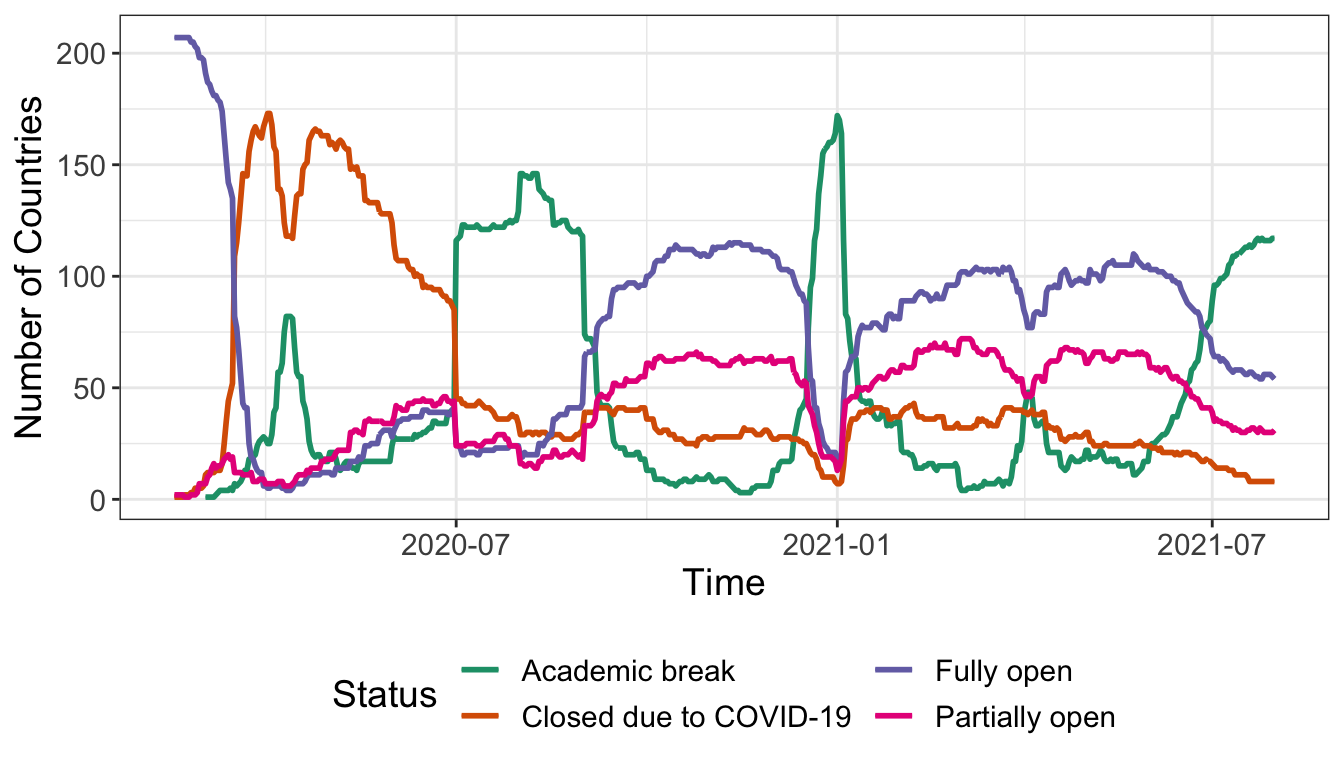
\includegraphics[width=1\textwidth]{figure/covidImpactWorld-1} 

}

\caption{Global tracking of COVID-19 caused school closures and re-openings}\label{fig:covidImpactWorld}
\end{figure}

\begin{figure}[h]

{\centering 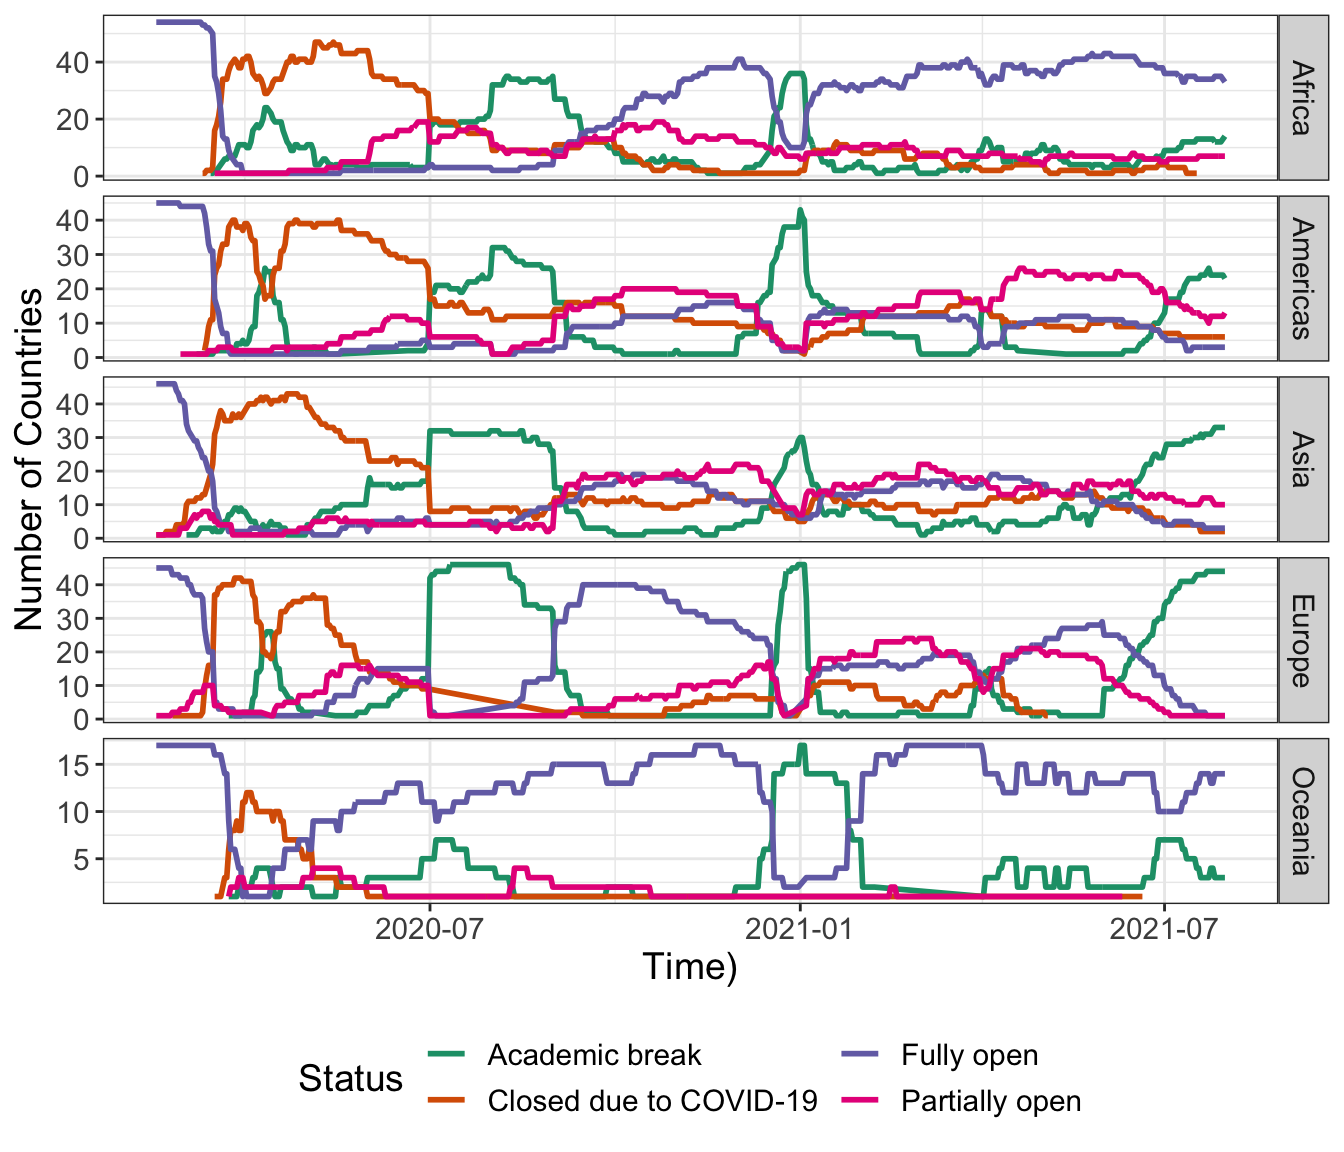
\includegraphics[width=1\textwidth]{figure/covidImpactContinent-1} 

}

\caption{Region wise tracking of COVID-19 caused school closures and re-openings}\label{fig:covidImpactContinent}
\end{figure}

The ongoing COVID-19 pandemic has brought the world to a standstill. Many sectors have been affected ever since the outbreak of COVID 19, worldwide. Among these many sectors education is one of the most affected sectors with a near-total closures of schools, colleges and universities, all around the world \autocite{daniel2020education}. Figures \ref{fig:covidImpactWorld} shows the evolution of global school closures and reopening since mid February 2020 \autocite{unesco2020covid}. With the start of the pandemic a near total closure of schools were observed all around the world. Over time, Africa and Oceania demonstrated better recovery in comparison to other regions with their increasing number of fully open schools where classes are being held exclusively in person (Figures \ref{fig:covidImpactContinent}).

\begin{figure}[h]

{\centering 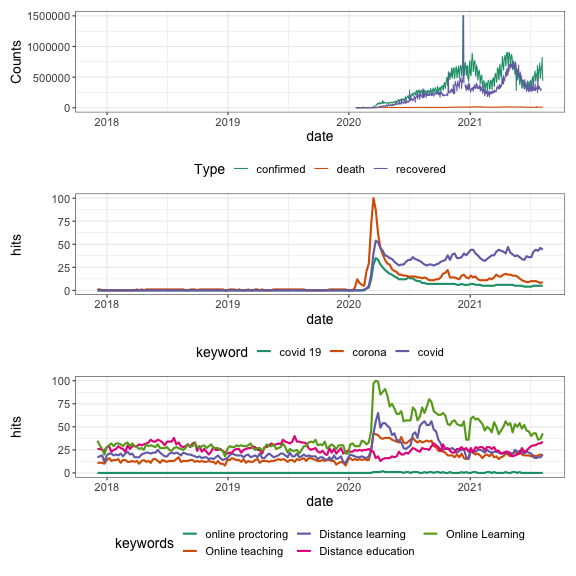
\includegraphics[width=1\textwidth]{figure/distanceLearningWorldAnalysis-1} 

}

\caption{Visualization of data from Goolge search trends. (a) COVID-19 cases worldwide (b) Google search trends of COVID-19 related terms (c) Google search trends of distance education related terms.}\label{fig:distanceLearningWorldAnalysis}
\end{figure}

Eventhough distance education has a long history that goes back to almost two centuries with significant modifications,
alterations, and addition in the process of delivery and communication \autocite{moore2011learning,spector2014handbook}, COVID 19 certainly made a new era of distance education while encouraging various stakeholders of education to take the concept of distance education seriously \autocite{richmond2020critical}. Sudden unexpected movement from classrooms to home schooling at large scale made students, teachers and parents vulnerable, leading to millions of education related internet searches being performed during the period of COVID 19 pandemic (Figures \ref{fig:distanceLearningWorldAnalysis}) \autocite{carter2021teacher}. Surprisingly, the search spikes of distance education related searches (Figure \ref{fig:distanceLearningWorldAnalysis} (c)) coincide with increasing Covid-19 counts (Figure \ref{fig:distanceLearningWorldAnalysis} (a)) and related internet searches (Figure \ref{fig:distanceLearningWorldAnalysis} (b)), eventhough distance education has a long history in contrast to Covid-19 pandemic.

The speed of the physical classroom closures and the rapid move to online delivery of education allowed little time for planning or reflection on potential risks that could happen to its various stakeholders: teachers, students and parents. Teachers were not fully aware of their obligations and how to maintain connections with students to support thier learning. Lack of preparation, lack of tools and techniques for distance education, lack of awareness of the availability of the existing tools and techniques and their effectiveness, lack of interaction and communication with the students, lack of awareness of students' ongoing problems were some of the major issues they encountered during COVID 19 pandemic. Students on the other hand who tend to have fewer educational opportunities beyond schools and universities severely affected from this sudden unexpected movement. Further, the impact was not limited to students' learning but also to other aspects of their lives such as student debt, digital exclusion, lack of technology, lack of access to internet-enabled device or a stable internet connection, long-term educational disengagement, poor nutrition and food insecurity, increased psychological challenges, childcare problems, exploitation, school dropouts and lack of disability services, long-term educational disengagement, digital exclusion, poor technology management, increased psychosocial challenges, decreases in mathematical achievement, a lack of engagement, increased early marriages , psychosocial challenges \autocite{drane2020impact,daniel2020education,unescoadverse2020,richmond2020critical,carter2021teacher}. This also put an extra burden on parents, specially with limited education and resources, as they were expected to facilitate the required learning environment at home. Working parents also found it difficult to work during school closure due to childcare obligations that result from unexpected school closures. Further, every single step including planning, developing new tools and techniques, conducting awareness programmes about distance education, shifting towards distance education, happened through online, due to the unexpected massive global shutdown. This situation left internet as the only medium to support all these educational processes.

In response to this gray situation and urgent requirement of massive transformation from physical classroom to virtual learning environment, UNESCO took immediate and timely action by publishing a long list of distance learning solutions that can be used to facilitate student distance learning during the period of school closure. There are many different distance learning solutions. Yet very little is known about the uptake of different solutions or about their effectiveness. The design of different types of distance learning solutions can depend on the learning objective, target audience, access, and type of content \autocite{moore2011learning}. However, getting familiar with all these available distance solutions is not feasible or practical due to limited time availability and need of urgent responses. According to \textcite{carter2021teacher}, for educators to continue to teach inclusively, they need support to connect with the students through a variety of strategies so that students feel not only connected to their teachers, but to the subject matter being taught.

Connectivity, flexibility and ability to promote varied interactions are some critical aspects, educators consider when selecting distance education solutions. Further, according to \textcite{ahn2006utilizing}, the popularity of a product can also greatly influence consumer purchasing decisions as popularity can indicate the prominence of the product in the market, its usability and its impact. Further, according to \textcite{willis2020using}, developers also tend to improve their products and services in response to increasing online search. Therefore, the internet represents a great opportunity to learn about public attention towards a product or service. It is also a way to narrow down the search space and thereby identify most suitable product and services that meets customer needs.

Google Trends is an open source web analytics tool that allows users to interact with Internet search data, which can provide deep insights into population behavior \autocite{nuti2014use}. As there is still the main struggle as to what technologies should be used to facilitate student learning, in this study we test whether the Google Analytics search index series can be used as a proxy of the popularity and the public interest in different distance education solutions. In line with that, this paper makes three fundamental contributions to distance education by exploring three main questions: (1) What is the impact of COVID 19 pandemic on education? (2) What solutions are in place to meet the need of distance education in terms during COVID 19 pandemic? (3) Which distance learning solutions have a wide attention and public interest during the COVID-19 pandemic?
We primarily analyze quantitative digital footprint data on the internet from December 2019 to August 2021. The resulted google trend footprint provides a fast first step to identify the most popular distance education tools available for different education purposes. It also allows the teachers to narrow down the search space and deepen their exploration on prominent distance education solutions to support their online teaching. Further, identifying most popular tools and techniques will allow everyone to focus on those methods and develop a sustainable learning environment by advancing the existing features.

Quality education is essential to sustainable development and it is a key United Nations (UN) sustainable development goal. Having the right tool is imperative to successful completion of a task at hand. The findings of this study provides an initial guidance to select a right tool. Therefore, the findings of this study directly contribute to UN's sustainable development goals of quality education.

The remainder of this paper is organized as follows. Section 2 presents the related work to lay the foundation for the Google trend footprint analysis of different distance learning solutions. Section 3 presents the methodology followed in the study. Section 4 includes results and discussion. Section 5 concludes the article and presents future research directions.

\hypertarget{background}{%
\section{Background}\label{background}}

The term distance education is known by a variety of names. The terms such as distance learning, e-Learning, online learning environments, home study, independent study, external
study, correspondence education, off campus study, open learning and open education are used commonly and interchangeably \autocite{moore2011learning}. It often describes the effort of providing access to learning for those who are geographically distant. The definition also stated that distance education uses emerging media and associated experiences to produce distributed learning opportunities. Few common features found in all these terms is they all involve some form of instruction occurs between two parties; learners and teachers, different times, places and/or varying forms of instructional materials \autocite{moore2011learning}. There are different types of interactions that facilitate learners to construct knowledge in distance education environments. These are learner--content interactions, learner--instructor interactions, learner--learner interactions and learner--interface interaction \autocite{wallace2003online}.

Google Trends, is a freely accessible website sponsored by Google that analyzes spatio and temporal patterns of search queries in Google Search, across various regions, subject domains and languages \autocite{carneiro2009google}. Therefore, Google trends provide a quantifiable and valuable measure of emerging public concerns and trending topics together with their geographic distribution \autocite{alicino2015assessing,cook2011assessing}. According to \textcite{jarynowski2020perception} the public concerns on different matters can also take an epidemic nature starting with the phase of growing interest which is known as ``early adoption'', to the phase of general interest which is known as ``majority'' to eventually lose popularity which is known as ``lagers stage''. Figure \ref{fig:distanceLearningWorldAnalysis} also confirms this life cycle explanation.

The use of google trend search queries has become a popular data source in monitoring and modeling the dynamics of different domains such as disaster management \autocite{kam2019monitoring}, transportation \autocite{willis2020using}, business \autocite{chumnumpan2019understanding} and health care \autocite{nuti2014use,alicino2015assessing,arora2019google,carneiro2009google,cook2011assessing} as it provides data about social phenomena in a more timely manner than traditional data collection processes \autocite{vaughan2014web}. According to the study conducted by \textcite{willis2020using} on taxi preferences found that online queries can provide a proxy of quality of taxi services and thereby provide a means to investigate service quality and public concerns on the service provided. In November, 2008, Google launched an internet-based surveillance tool, Google Flu Trends (GFT), that uses aggregated Google search data to provide a near real-time support in predicting influenza outbreaks \autocite{cook2011assessing}. Several recent studies have also been conducted to investigate the relation between Google search trend patterns and the COVID-19 related concerns \autocite{husnayain2020applications,effenberger2020association}. The study conducted by \textcite{husnayain2020applications} focuses on search terms related to the coronavirus, handwashing, and face masks to monitor public restlessness toward COVID-19. However, there are only a limited number of research attempts related to education section using Google trend search query data \autocite{vaughan2014web}. The study conducted by \textcite{vaughan2014web} have used google trend search queries to predict academic fame by testing the correlation between search volume data and university ranking data. \textcite{kansal2021google} have used a text mining approach to identify emerging patterns of words and phrases during COVID-19 pandemic, keeping education prospects as the focus. However, their study was limited to a small number of learning platforms. However, according to \textcite{moore2011learning} the design of different types of learning environments can depend on the learning objective, target audience, access (physical, virtual and/or both), and type of content. Therefore, this study provides a detailed investigation on distance education solutions focusing on different distance learning needs. In contrast to the work in \textcite{kansal2021google}, the work in our paper has a very specific focus: the distance learning solutions for various education purposes.

Eventhough google trend search quiries provide massive amount of data, more care should be given when utilizing it as a research tool. It may contain inaccuracies \autocite{carneiro2009google}. According to \textcite{nuti2014use} the data retrieval process should be transparent. This will increase the trustworthiness of both the results and the generalizability of the findings. Furthermore, researchers should clearly document the rationale and data retrieval process to ensure the reproducibility of results \autocite{nuti2014use}. .

\hypertarget{methodology}{%
\section{Methodology}\label{methodology}}

To identify the impact of covid 19 on education, data on the evolution of school closures and re-openings was obtained from a repository maintained by UNESCO \autocite{unesco2020covid}. Data related to Covid-19 cases was retrieved from the R software \autocite{rsoftware} package \texttt{coronavirus} \autocite{coronavirusr}. The package pulls data from the Johns
Hopkins University Center for Systems Science and Engineering (JHU CCSE) data repository \autocite{dong2020interactive}.

In this work we also used Google Analytics search index series as a measurement proxy to investigate emerging evidence about distance learning and the popularity and the public interest in various distance education solutions. We used weekly Google Analytics search index series of various distance learning solutions during covid-19 pandemic. We limited all of our searches to the period from 1 December 2019 to 15 August 2021 to match the period of Covid-19 pandemic. Through this we wanted to capture the volume of interest in the public realm about distance education solutions and how this changes over time. We also studied the cross correlation between weekly web searches and the weekly cases of covid-19.

Google Trends determines categories based on search patterns. According to \textcite{vaughan2014web} more relevant accurate data can be obtained by limiting the search in Google Trends to a specific category as it helps to reduce noise in the data. In this work our focus was given to education category. Google Trends does not provide the absolute search volume of a given search term. Instead it provides a relative search volume of a particular term adjusted according to the total searches of the geography and time range it represents. The resulted series scale from 0 to 100, where each data point in the series represents the search interest relative to the highest point on the series for the selected region and time. \autocite{alicino2015assessing,vaughan2014web}. A value of 100 represents the peak popularity of the term.

It is important to decide what term to search for in Google Trends as different terms have different search volumes. In the past literature several strategies have been used to select suitable search terms for a given study. Some studies have selected search terms based on intuition and some through brainstorming processes \autocite{vaughan2014web}. In this study our choice of search term took into account the list of distance learning solutions published by UNESCO \autocite{unesco2020DLsolutions}.
Eventhough, the solutions they had recommended do not carry their explicit endorsement, they tend to have a wide reach, a strong user-base and evidence of impact \autocite{unesco2020DLsolutions}. Different solutions are categorized based on distance learning needs. For each keyword, the worldwide search queries were performed with a keyword being used as the ``search term''. That allowed us to search the exact string of text typed by the user. However, according to \textcite{vaughan2014web}, short forms or acronyms had higher search volumes than the corresponding complete names, in general. However we did not use the acronym in this study, as our focus is on specific tools and techniques available in the market to fulfill distance education needs and acronyms could be confused with another entity.

Google Trends allows to search for up to five queries each time \autocite{vaughan2014web}. We did our analysis under 11 sub segmentations namely, digital learning management systems, systems built for use on basic mobile phones, systems with strong offline functionality, Massive Open Online Course (MOOC) Platforms, self-directed learning content, mobile reading applications, Collaboration platforms that support live-video communication, tools for teachers to create of digital learning content, external repositories of distance learning solutions, tools for online proctoring and Resources to provide psychosocial support. The segmentation was mainly motivated by the list of distance learning solutions published by UNESCO in response to Covid 19 pandemic.

In google trends, it is possible to search for only up to five queries at a time. Therefore, under each segmentation we entered up to five distance learning tools at a time and recorded their relative ranking scores. An iterative pairwise comparison was first used to identify the series that has highest search volume during the study period. Through this iterative process of relative comparison, we were able to identify the tool with the highest relative ranking score. Then the relative ranking scores for all the other tools in the given segmentation was obtained relative to the previously detected series with the highest ranking scores \autocite{vaughan2014web}.

Both visual and analytical approaches were used to analyse the changes in web search queries at the global level over the entire period of the Covid-19 pandemic to identify the emerging evidence about the impact of COVID-19 pandemic on distance education. We also evaluated the relationship between weekly web searches and the number of weekly global cases of covid-19. Cross correlation analysis and the dynamic time warping algorithm \autocite{giorgino2009computing} were performed to investigate the relationship and similarities between the signatures of covid-19 related search volume data and distance education related search volume data.

\hypertarget{results-and-discussion}{%
\section{Results and Discussion}\label{results-and-discussion}}

Search volume index graphs for Covid 19 related terms worldwide (Figures \ref{fig:distanceLearningWorldAnalysis} (b)) shows that the highest peak coincided with the start of the pandemic. Surprisingly, the search volume index graph for distanced education related terms (Figures \ref{fig:distanceLearningWorldAnalysis} (c)) also shows a similar spike at the start of the pandemic. According to \textcite{moore2011learning}, ``distance education'' is the most renowned descriptor used when referencing distance learning. However, both \textcite{benson2002usability} and \textcite{conrad2002deep} introduced ``online learning'' as the most ``recent version'', ``never version'' and ``improved version'' of distance learning. The google search trend pattern corresponds to the term ``online learning'' (Figures \ref{fig:distanceLearningWorldAnalysis} (c)) confirms the above claim as it is the most searched distance education related term throughout Covid-19 pandemic. Despite quantitative differences in terms of relative search volume, the series generated by the two terms ``Distance learning'' and ``online teaching'' demonstrate a similar trend during the study period. Covid-19 related web searches declined in the months after the WHO announcement of the Covid-19 pandemic, despite the increase in Covid-19 cases. A similar decline could be detected in distance education related terms. further, a second was observed only in education related terms after the WHO announcement of the Covid-19 pandemic. This could be due to the near total closures of schools happened with the declaration of Covid-19 as a pandemic.

\begin{figure}[h]

{\centering 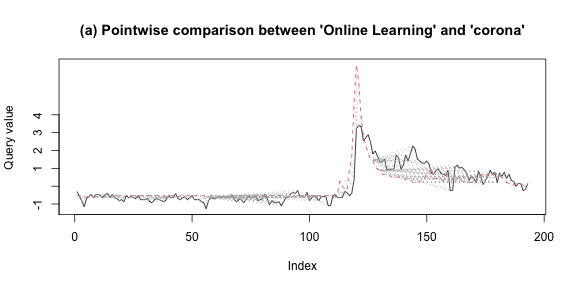
\includegraphics[width=1\textwidth]{figure/dtw1-1} 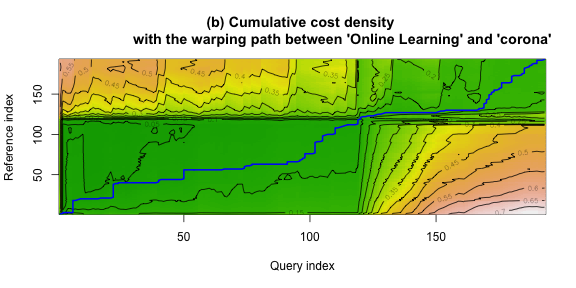
\includegraphics[width=1\textwidth]{figure/dtw1-2} 

}

\caption{Visualization of Dynamic Time Warping Alignments between 'online learning' and 'corona'}\label{fig:dtw1}
\end{figure}

\begin{figure}[h]

{\centering 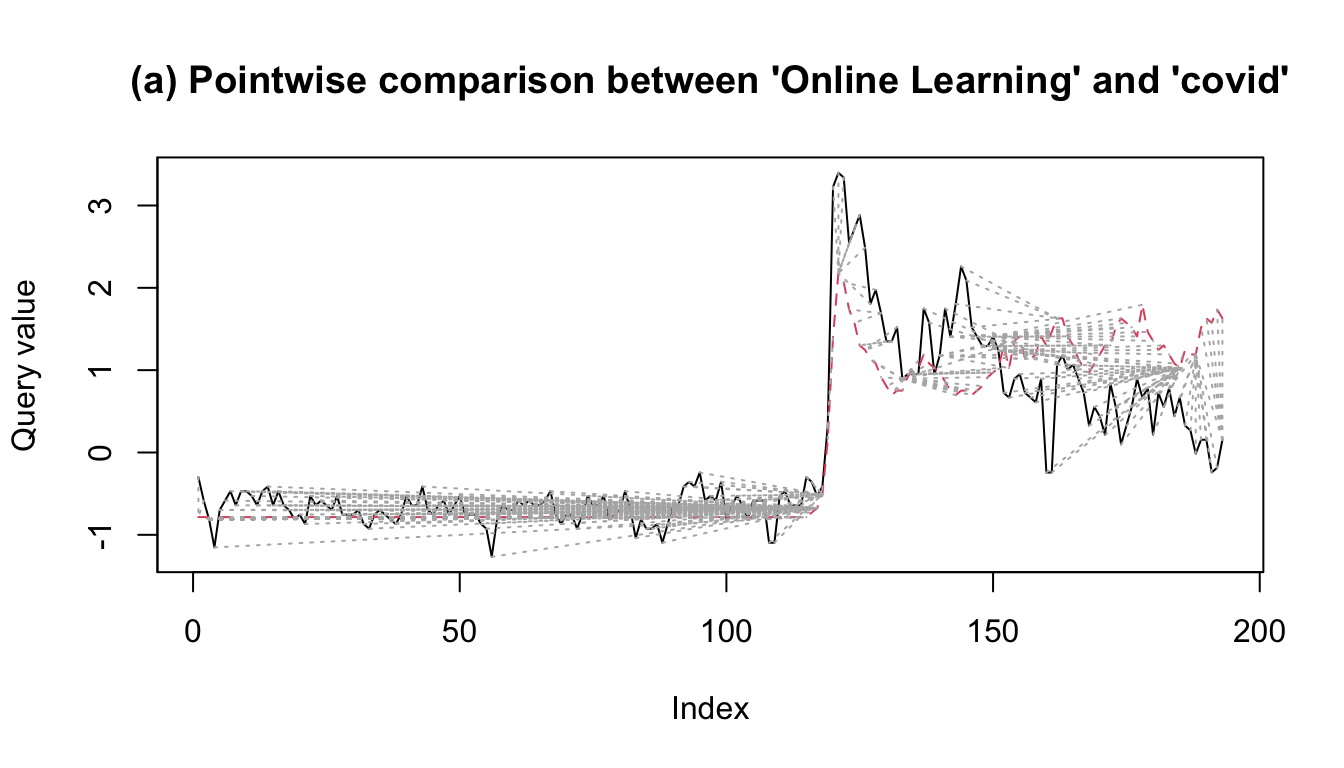
\includegraphics[width=1\textwidth]{figure/dtw2-1} 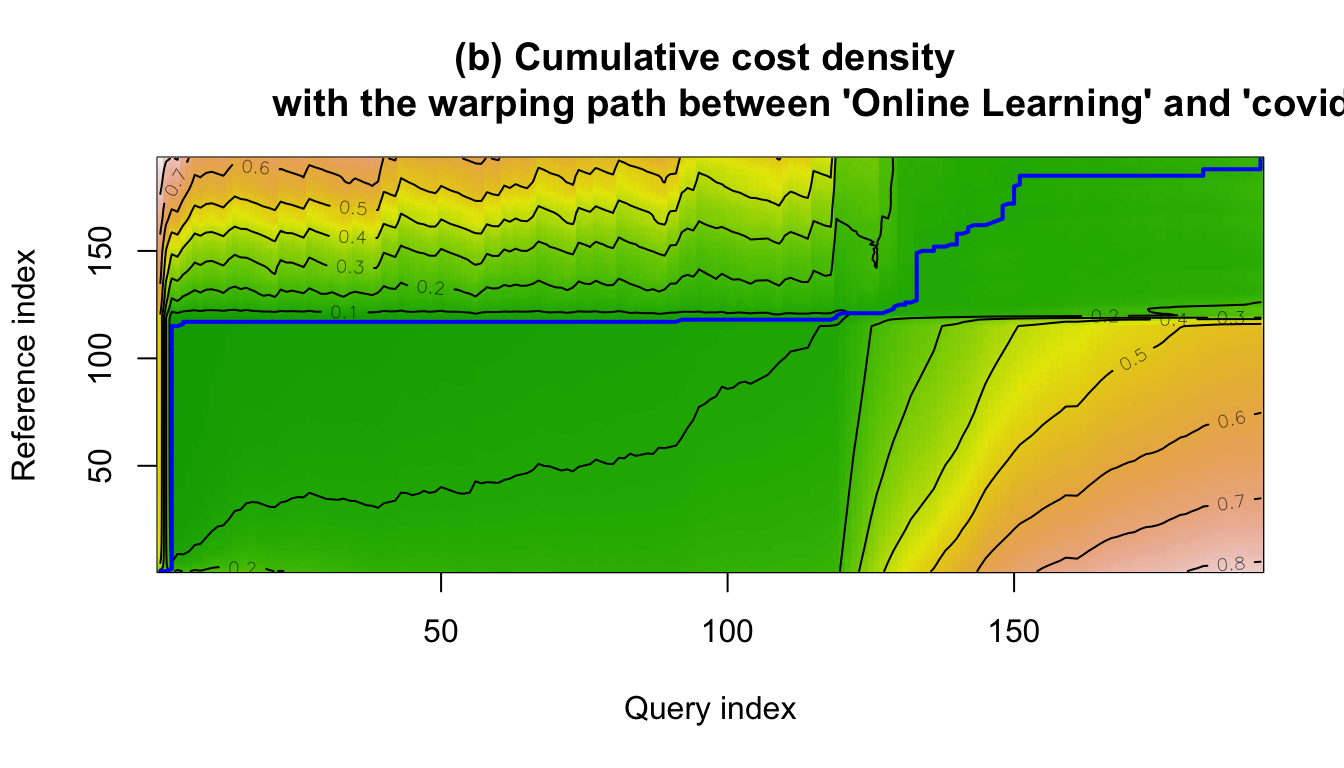
\includegraphics[width=1\textwidth]{figure/dtw2-2} 

}

\caption{Visualization of Dynamic Time Warping Alignments  'online learning' and 'covid'}\label{fig:dtw2}
\end{figure}

The pairwise comparison performed using Dynamic Time Warping algorithm. Under this approach the two time series are stretched or compressed locally in order to make one resemble the other as much as possible. The distance between the two series is then computed by summing the distances of individual aligned elements \autocite{giorgino2009computing}. Two pairwise comparisons, ``corona'' with ``online learning'' and ``covid'' with ``online learning'' were conducted to see the impact from covid 19 on distance education. Both pairwise comparison show a significant areas of overlap and a similar dynamic pattern (Figures \ref{fig:dtw1} (a) and \ref{fig:dtw2} (a)). The normalized distance between the two series in the two comparisons are 0.1326197 and 0.1828299, respectively. This also provides further confirmation for the similarity of the google trend search profiles.

The entirety of the blue warping path flows through green pastures further confirms the similarity between the search pattern related to covid 19 and distance education (Figures \ref{fig:dtw1} (b) and \ref{fig:dtw2} (b)). The orange volcanic topography that highlights regions of nonalignment of series in question if mapped through this region demonstrate a significant difference in online search behaviours before and after covid 19 pandemic (Figures \ref{fig:dtw1} (b) and \ref{fig:dtw2} (b)).

The degree of digression of blue line from the ideal 45-degree straight line indicates a dissimilarity of the two time
series (Figures \ref{fig:dtw1} (b) and \ref{fig:dtw2} (b)). In 2019 the infection was recognized as a virus which is genetically related to the corona virus responsible for the Severe Acute Respiratory Syndrome (SARS) outbreak of 2003 which infected over 8,000 people from different countries that resulted more than 700 deaths worldwide. By the time it was know as ``corona'', it was not a global concern and was mostly limited to China. During that time people did not pay much attention to online learning as conventional classroom learning approach was the most popular teaching learning strategy prior to Covid 19 pandemic all around the world. This is evident from the rough flat line from approximately 120 to 170 on the Query Index axis.

Later with the spread of the virus worldwide, WHO named it as COVID-19 (COrona VIrus Diagnosed in 2019) and then declared it as a pandemic on March 11, 2020. With that, a near total closure of schools were observed all around the world (Figures \ref{fig:covidImpactWorld}). With this sudden unexpected movement, online learning also became an equally important global concern, similar to covid 19 pandemic. This similar behaviour in public attention towards both aspects is confirmed by the blue line that fall on near 45-degree line from approximately 120 to 150 on the Query Index axis. This also confirms the impact of covid 19 on distance education and online learning.

Then, a cross correlation analysis was performed to estimate the lag between covid 19 related terms and the distance education related terms (Figures \ref{fig:ccfAnalysis}). A close relationship was evident between covid related search patterns and the search patterns of the terms ``Online learning'', ``Distance learning'' and ``Online teaching''. The significant cross-correlation coefficients at lag zero confirms contemporaneous relationship between the covid related search terms and distance learning related search terms. The significant cross correlation values at lag one or two also confirms the sudden impact of covid 19 pandemic on distance education related public concerns (Figures \ref{fig:ccfAnalysis} (a) - (c) and (f) - (h)). However, no significant synchronization was observed between the Covid 19 related search trends and the search patterns of ``distance education'' or ``online proctoring'' (Figures \ref{fig:ccfAnalysis} (d), (i), (e), (j)).

\begin{figure}[h]

{\centering 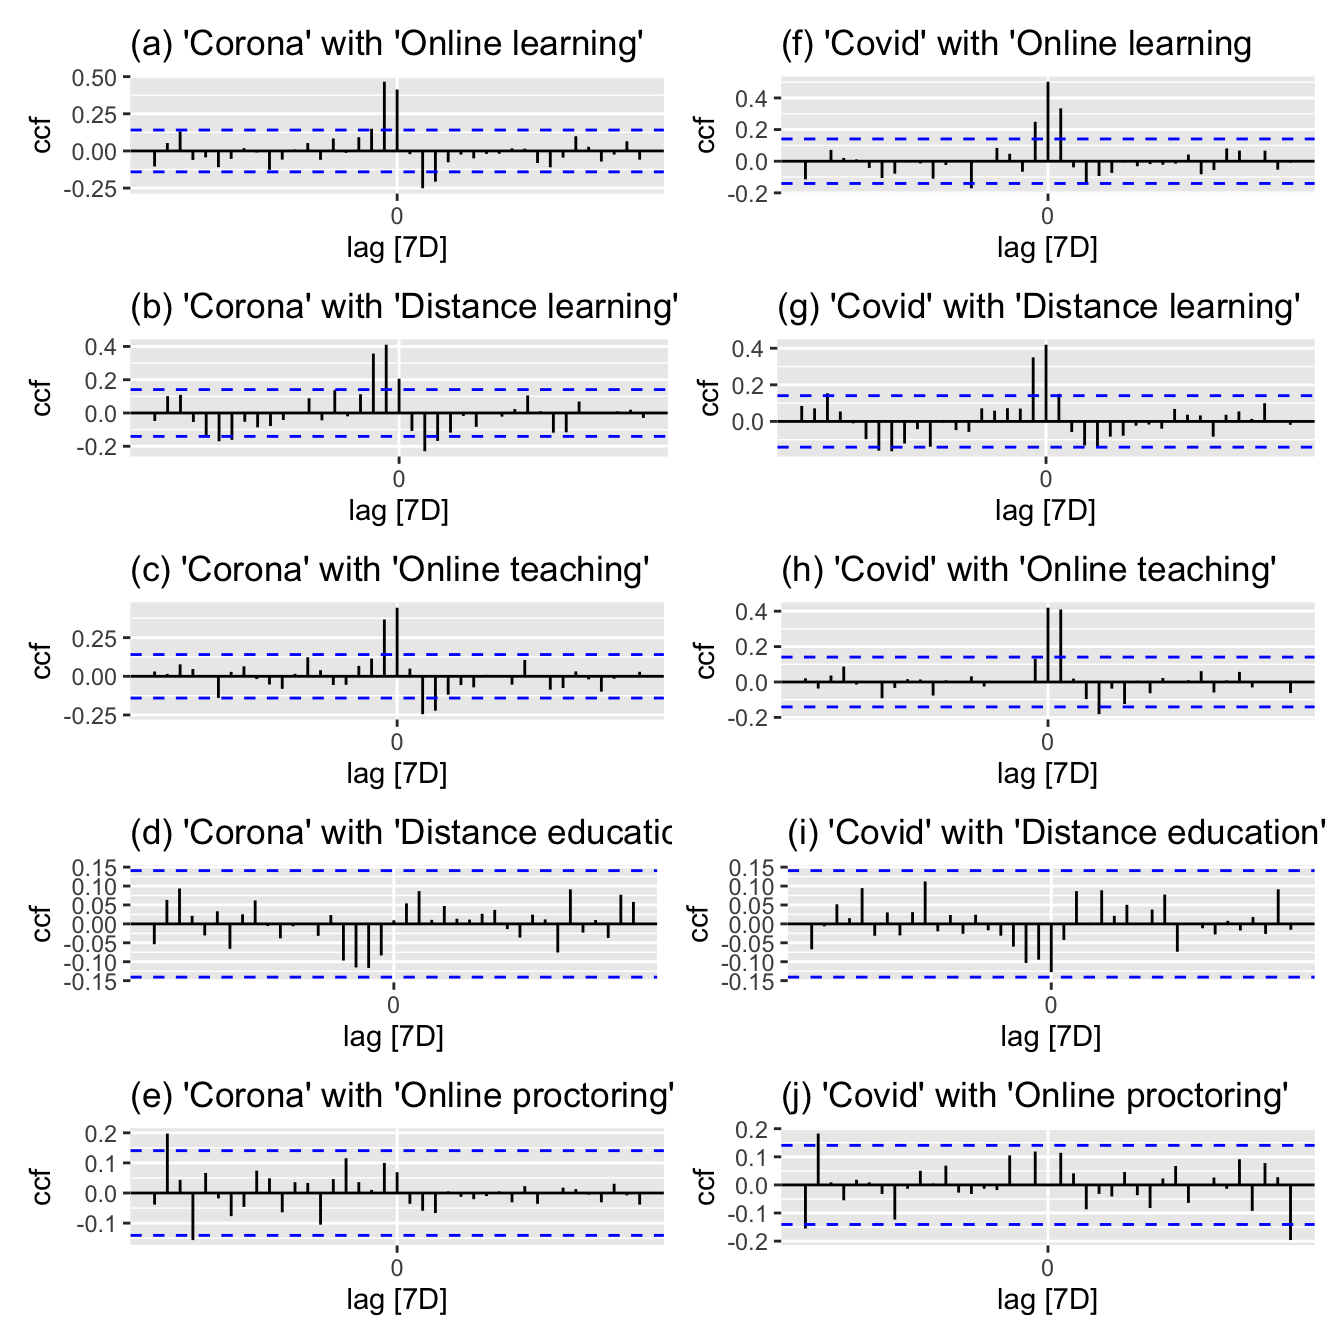
\includegraphics[width=1\textwidth]{figure/ccfAnalysis-1} 

}

\caption{Cross-correlation analysis between distance learning related online search terms and covid 19 relate online search terms during Covid-19 pandemic}\label{fig:ccfAnalysis}
\end{figure}

The list of distance education solutions published by UNESCO provides many different distance education solutions for different education purposes. Figure \ref{fig:plot1} and Figure \ref{fig:plot2} provide a Google trend footprint that can be used as a proxy for measuring global attention towards different distance learning solutions. This provides a fast first step to identify the most popular tools available for different educational purposes. Under each and every category Figure \ref{fig:plot1} (a) - (e) and Figure \ref{fig:plot2} (f) - (j), one or two tools have got a significantly higher level of attention in comparison to the remaining options available undue the same category. The time series across multiple panels are not comparable as they represent ``relative'' search volume of given terms and they are comparable only with a given panel. The value 100 is also not comparable across multiple panels and indicates the maximum popularity for the term within each category.

Under digital learning management systems ``Google Classroom'', which helps teachers and students connect remotely, communicate and stay-organized, has got a wide attention and public interest during covid 19 pandemic (Figure \ref{fig:plot1} (a)). This might be due to it's easy and fast setup and usage \autocite{sudarsana2019use}. Under systems built for use on basic mobile phones, both `kaiOS' and `Ubongo' have received a wide attention during the pandemic (Figure \ref{fig:plot1} (b)).
`KaiOs' has the ability provide smartphone capabilities to inexpensive affordable devices and thereby helps open portals to learning opportunities. `Ubongo' has also received a considerable attention, eventhough its target groups are school-age children and their parents in Africa. It facilitates localized, multi-platform Entertainment-Education to African families at low cost and massive scale and is available in both Kiswahili and English. A significant peak in `Ubongo' series can be observed during 2020 year end academic break in Africa (Figure \ref{fig:covidImpactContinent}).
Under systems with strong offline functionality, `Kolibri', which is available in more than 20 languages, supporting universal education, has got a considerable attention during covid-19 pandemic (Figure \ref{fig:plot1} (c)) as the tool focuses on facilitating learners living in underserved contexts where the internet is costly, unreliable, or unreachable. The can be a huge relief for financially distressed families during Covid-19 pandemic. Under Massive Open Online Course (MOOC) platforms, `Canvas', which provides free access for teachers to facilitate learning and professional development, has got a considerable attention in comparison to other options available (Figure \ref{fig:plot1} (d)). `Udemy' has got the second highest attention. However, `Canvas' has received far more attention than `Udemy'. Under self-directed learning content `Quizlet' has got a considerably high attention throughout the pandemic in comparison to the other options available under the same category (Figure \ref{fig:plot1} (e)). It provides learning flashcards, AI based learning assistant and games to support student learning in multiple subjects and languages. The second highest option only provides support for language learning. `Quizlet'`s ability provide support for multiple subject might be the reason for it to outperform it competitor in the market. Under mobile reading applications, 'Reads', which provides digital stories with illustrations in multiple languages has consistently being the most popular option (Figure \ref{fig:plot2} (f)). Under collaboration platforms that support live-video communication, both `WhatsApp' and `Zoom' had got a considerable attention at the start of the pandemic in March 2020 (Figure \ref{fig:plot2} (g)). However, `WhatsApp' has outperformed `Zoom' overtime through with increasing public attention during the pandemic. In contrary, the global attention towards `Zoom' has decreased over time. `Teams' has also got considerable attention in comparison to the other remaining options available int he market. Under tools for teachers to create of digital learning content, `Trello' which provides a visual collaboration platform for teachers for coursework planning, classroom organization and collaboration, has received a wide attention during the pandemic. `Nearpod', that promotes active learning and student engagement through informative and interactive learning activities has also got a considerable attention during the pandemic (Figure \ref{fig:plot2} (h)). A significant peak can be observed in the `Nearpod' series, during the first academic break. Under external repositories of distance learning solutions, both `Brookings' and `UNHCR' have got a significant global attention (Figure \ref{fig:plot2} (i)). `Brookings' provides a large catalogue of learning innovations eventhough its focus is not limited to distance learning solutions. `UNHCR' also provides an extensive list of distance learning solutions from the United Nations agency for refugees. Student assessment is vital in ensuring the quality of education. However, due unexpected sudden school closure, administering examinations at a distance became a major concern. Under tools for online proctoring, `Pearson VUE' which provides computer based testing services in
over 150 countries worldwide with more than 5,000 authorized test centers has got a considerably high public attention during the pandemic (Figure \ref{fig:plot2} (j)).

At the start of the pandemic in March 2020, a significant peak of public attention can be observed in both 'digital learning management systems (Figure \ref{fig:plot1} (a)) and collaboration platforms that support live-video communication (Figure \ref{fig:plot2} (g)). These peaks aligns with the near-total closures of schools due to covid 19 in Figure \ref{fig:covidImpactWorld}. The major concerns that arise with the unexpected sudden movement from physical classroom to virtual learning environment, such as lack of experience to connect and share learning materials with students could be the reasons for this notable public attention towards these two aspects. Further, a significant peak can be observed in digital learning management systems (Figure \ref{fig:plot1} (a)), Massive Open Online Course (MOOC) Platforms (Figure \ref{fig:plot1} (d)), Self-directed learning content (Figure \ref{fig:plot1} (e)), collaboration platforms that support live-video communication (Figure \ref{fig:plot2} (g)) and tools for teachers to create of digital learning content (Figure \ref{fig:plot2} (h)), immediately after the academic break in August, 2020 (Figure \ref{fig:covidImpactWorld}). The inability to reopen school fully due to the increasing Covid-19 cases worldwide and the need of urgent responses to connect with students to somehow facilitate their learning could be the reason for this considerable public attention around August, 2020.

\begin{figure}[h]

{\centering 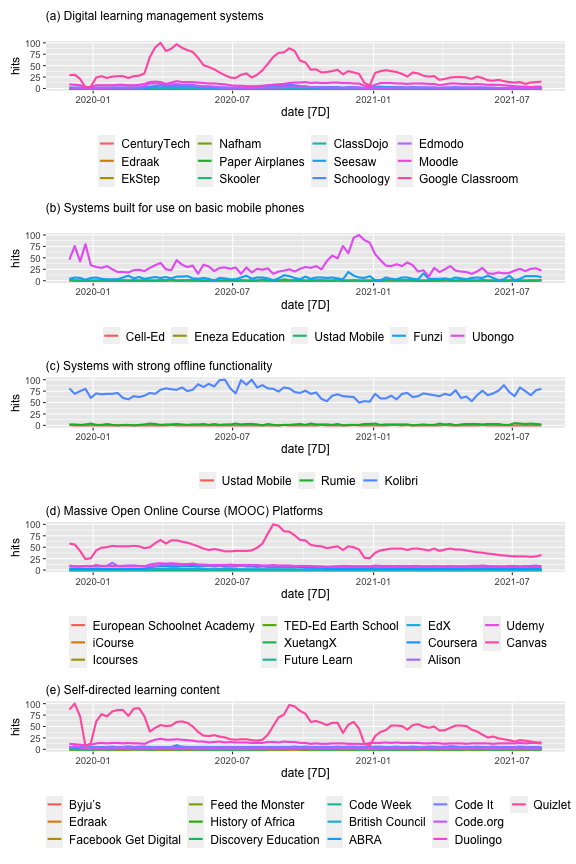
\includegraphics[width=1\textwidth]{figure/plot1-1} 

}

\caption{Google search trends footprint analysis}\label{fig:plot1}
\end{figure}

\begin{figure}[h]

{\centering 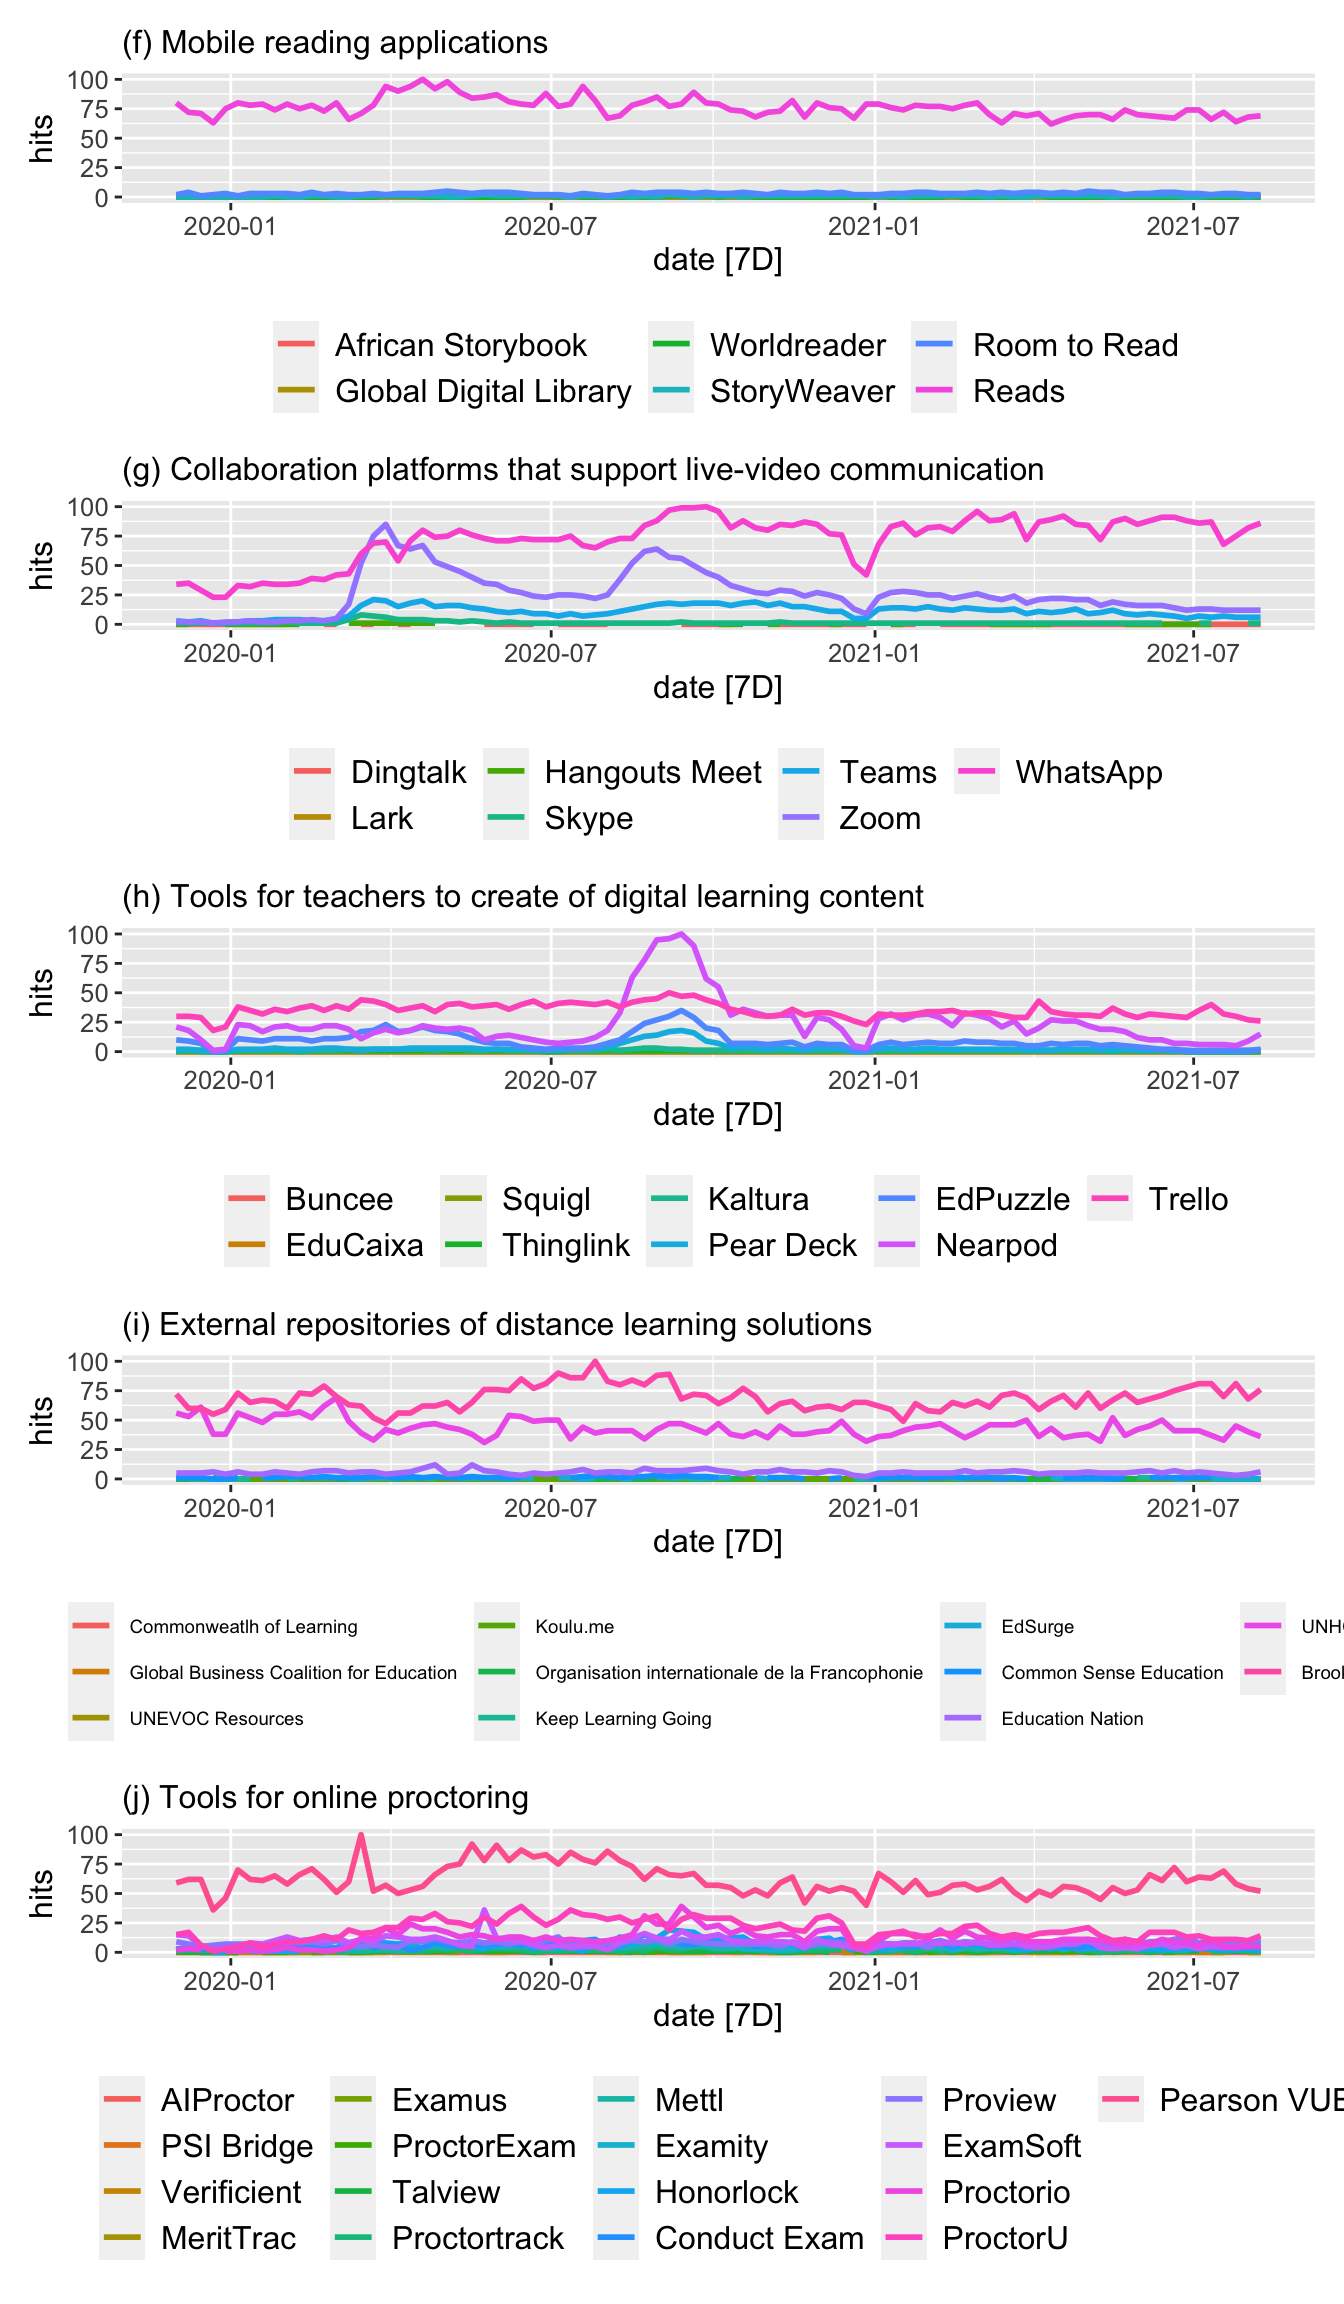
\includegraphics[width=1\textwidth]{figure/plot2-1} 

}

\caption{Google search trends footprint analysis}\label{fig:plot2}
\end{figure}

The attention in the education sector is low compared to all category. However a significant peak can be observed during the first academic break after declaring Covid 19 as a pandemic. Similar peak can be observed in 2021 . But that significant compared to 2020 peak.

\begin{figure}[h]

{\centering 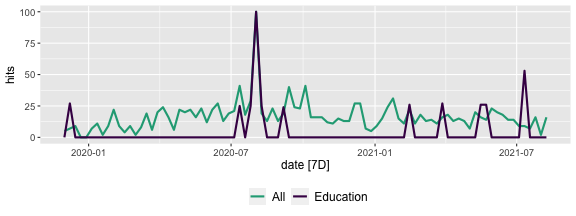
\includegraphics[width=1\textwidth]{figure/psychosocialSupportAnalysis-1} 

}

\caption{Goolge search trend of the term 'Psychosocial support' under 'All categories' and 'Education' search category}\label{fig:psychosocialSupportAnalysis}
\end{figure}

Good psychosocial support is also vital to improve both students' and teachers' mental health and well-being during a pandemic. This is evident in Figure \ref{fig: psychosocialSupportAnalysis} from the two sudden spikes in the search volume index graphs of the term `Psychosocial support' which correspond well with the academic breaks in August in both years 2020 and 2021, under `Education' category. This highlight the urgent need of attention and solutions towards these aspects. This type of an analysis based on secondary data is very vital as these types of aspects can be easily overlooked due to the lack of connection and communication between students and educators during school closures.

\hypertarget{conclusions-and-further-work}{%
\section{Conclusions and Further work}\label{conclusions-and-further-work}}

In this study we investigated whether the Google trend search queries can be used as a proxy of the popularity and the public interest in different distance education solutions. This study is the first detailed analysis of web search behaviour related to distance learning solutions, both in quantitative and qualitative terms during covid 19 pandemic. A few previous published studies \autocite{vaughan2014web,kansal2021google} have investigated Google trend search queries related to education, but only with a limited number of search terms or different focuses.

Our findings suggest that web search interest in distance learning solutions at the global was strongly influenced by the Covid-19 pandemic. Google trend search queries showed a strong cross correlation between covid-19 related search terms and distance education related search terms. The high popularity and increasing public attention towards different distance learning solutions during Covid-19 pandemic was also investigated through a detailed google trend footprint analysis. The findings will help the educators to narrow down their search space and thereby select prominent options available in the market for different education purposes. According to \textcite{wallace2003online}, the learning tools can have a significant impact on how students engage in online learning. The finding will also helpful for developers to identify their competitors in the market. High cost involved with different distance learning solutions, lack of financial support/funding and lack of understanding about the existing distance learning solutions are some of the major issues the educational institutions face with the covid-19 pandemic. These findings offer important insights to various stakeholders of education to make better decision with less effort and time.

Google Trends only captures the search behaviour of a a sub population with Internet access, eventhough it is the most common worldwide search engine. Our study focused on global attention toward distance learning solutions during Covid-19 pandemic. Therefore, care should be given when generalizing these findings to different regions or different time periods, as different regions can have different market orientation and seasonal requirements. This can lead to variations in the search output and in turn the study findings for different regions and time frames. Further, Google Trends data were not available as absolute values and available only in the form of relative volume. Therfore the scores ranges from 0 to 100 do not allow the researchers to make meaningful comparisons across different education needs. Further investigation is needed at national and regional level to identify the specific measures that can be taken to ensure the quality of distance education at national and regional level.

\hypertarget{supplementary-materials}{%
\section*{Supplementary Materials}\label{supplementary-materials}}
\addcontentsline{toc}{section}{Supplementary Materials}

\textbf{Data and scripts}: Datasets and R code to reproduce all figures in this article (\url{https://github.com/pridiltal/Covid19_Online_Teaching_paper}).

\hypertarget{acknowledgment}{%
\section*{Acknowledgment}\label{acknowledgment}}
\addcontentsline{toc}{section}{Acknowledgment}

This work was carried out with the aid of a grant form UNESCO and the International Development Research Centre, Ottawa, Canada. The views expressed herein do not necessarily represent those of UNESCO, IDRC or its Board of Governors.

\printbibliography

\end{document}
